\documentclass[conference]{IEEEtran}
\usepackage[T1]{fontenc}
\usepackage{newtxtext,newtxmath}
\usepackage{booktabs,tabularx,array,multirow}
\usepackage{graphicx}
\usepackage{pgfplots}
\usepackage{placeins}
\usepackage{needspace}
\usepackage{url}
\usepackage{float}
\pgfplotsset{compat=1.18}
\setlength{\tabcolsep}{3pt}
\renewcommand{\arraystretch}{1.12}
\newcommand{\safeSection}[1]{\Needspace{5\baselineskip}\section{#1}}
\newcommand{\safeSubsection}[1]{\Needspace{4\baselineskip}\subsection{#1}}
\newcommand{\paperheading}[1]{\Needspace{4\baselineskip}\vspace{1.1ex}\par\noindent\textbf{\MakeUppercase{#1}}\par\vspace{0.5ex}}
\newcolumntype{Y}{>{\raggedright\arraybackslash}X}
\newcommand{\pathcell}[1]{\begingroup\ttfamily\scriptsize\path{#1}\endgroup}
% Generated by generate_paper_figures.py from phase5_results/platform_trials.csv.
\newcommand{\ResultTableRows}{%
Discord & 45 & 45 & 100.0\% & 92.1--100.0\% & 0.0000 \\
WA Doc & 45 & 45 & 100.0\% & 92.1--100.0\% & 0.0000 \\
Telegram & 45 & 36 & 80.0\% & 66.2--89.1\% & 0.0274 \\
X & 45 & 0 & 0.0\% & 0.0--7.9\% & 1.0000 \\
Instagram & 45 & 0 & 0.0\% & 0.0--7.9\% & 1.0000 \\
WA Image & 45 & 0 & 0.0\% & 0.0--7.9\% & 1.0000 \\
\midrule
Overall & 270 & 126 & 46.7\% & 40.8--52.6\% & 0.5173 \\
}
\newcommand{\ComparisonTableRows}{%
Discord & 15 x 3 & 45/45 & success \\
WA Doc & 15 x 3 & 45/45 & success \\
Telegram & 15 x 3 & 36/45 & capacity / RS decode \\
X & 45 x 100 B & 0/45 & fixed-grid extraction \\
Instagram & 45 x 100 B & 0/45 & fixed-grid extraction \\
WA Image & 45 x 100 B & 0/45 & fixed-grid extraction \\
}


\title{ShadowPost: Measuring Native-JPEG DCT Steganography\\Survival Across Messaging and Social Platforms}
\author{\begin{tabular}{ccc}
\begin{minipage}[t]{0.31\textwidth}\centering\textbf{Arman Rizwan Khan}\\\textit{Dept. of Computer Science and Engineering}\\Priyadarshini College of Engineering\\Nagpur, Maharashtra, India\\arman.rkhan24@gmail.com\end{minipage} &
\begin{minipage}[t]{0.31\textwidth}\centering\textbf{Aditya Shakya}\\\textit{Dept. of Computer Science and Engineering}\\Priyadarshini College of Engineering\\Nagpur, Maharashtra, India\\adityashakya2712@gmail.com\end{minipage} &
\begin{minipage}[t]{0.31\textwidth}\centering\textbf{Divyani Dinkar Waikar}\\\textit{Dept. of Computer Science and Engineering}\\Priyadarshini College of Engineering\\Nagpur, Maharashtra, India\\divyaniwaikar2005@gmail.com\end{minipage}\\[1.2em]
\begin{minipage}[t]{0.31\textwidth}\centering\textbf{Aryan Manoj Terha}\\\textit{Dept. of Computer Science and Engineering}\\Priyadarshini College of Engineering\\Nagpur, Maharashtra, India\\aryanterha7@gmail.com\end{minipage} &
\begin{minipage}[t]{0.31\textwidth}\centering\textbf{Shreya Kamlesh Prasad}\\\textit{Dept. of Computer Science and Engineering}\\Priyadarshini College of Engineering\\Nagpur, Maharashtra, India\\shreyaprasad5367@gmail.com\end{minipage} &
\begin{minipage}[t]{0.31\textwidth}\centering\textbf{Rajshri Pote}\\\textit{Dept. of Computer Science and Engineering}\\Priyadarshini College of Engineering\\Nagpur, Maharashtra, India\\rajshri.pote@pcenagpur.edu.in\end{minipage}
\end{tabular}}

\begin{document}
\maketitle

\begin{abstract}
Platform image processing can invalidate a steganographic payload even when the embedding algorithm is correct. This paper presents ShadowPost, a native-JPEG DCT system that encrypts a message with AES-256-GCM, protects it with RS(48,32) error correction, and encodes bits through relative ordering of mid-frequency luminance coefficient pairs. The evaluation comprises 270 delivery trials representing six delivery modes across five platforms. Exact recovery was 45/45 for Discord attachments, 45/45 for WhatsApp documents, 36/45 for Telegram sendPhoto, and 0/45 for the tested X, Instagram, and standard WhatsApp image paths. These results characterize the tested account, client, and date configurations rather than the platforms universally.
\end{abstract}
\begin{IEEEkeywords}
image steganography, JPEG DCT, Reed-Solomon, AES-GCM, platform recompression, survivability benchmark
\end{IEEEkeywords}

\safeSection{Introduction}
A JPEG stego image is not delivered unchanged by many modern services. Upload pipelines may decode pixels, resize the image, quantize frequency coefficients, and encode a new JPEG. These operations are particularly damaging to methods that assume a stable 8 by 8 block grid. A useful system therefore needs both a robust embedding representation and measurements taken after real delivery.

ShadowPost addresses this problem as an end-to-end pipeline. The message is authenticated and encrypted before embedding; an error-correcting code provides bounded correction; and the hidden bits are represented by ordering pairs of native JPEG DCT coefficients. This study focuses on the delivery layer: how much of the encoded message remains recoverable after transmission through six practical channels.

\safeSection{Related Work and Design Position}
Digital steganography has historically been evaluated through imperceptibility, payload capacity, and resistance to statistical detection. Early data-hiding work established that a useful covert channel must consider both the embedding representation and the transformations expected during distribution [1]. Later JPEG research moved embedding from raw pixels toward quantized frequency coefficients because the JPEG codec itself operates on block DCT values [2], [4].

Robustness claims are strongly dependent on the distortion model. A method that survives a quality-factor change may still fail after resizing, cropping, color conversion, or a decode-and-reencode pipeline. Social platforms commonly combine several of these operations. Consequently, laboratory recompression at a known quality factor is not equivalent to uploading a file to a live service and decoding the derivative returned to a recipient.

Error-correcting codes are frequently added to robust data-hiding systems because small coefficient changes create isolated symbol errors. Reed-Solomon codes are appropriate for block-oriented payloads and provide a clear correction budget [5]. They do not, however, repair geometric desynchronization: if the receiver reads different spatial blocks, the resulting symbol stream is not a lightly corrupted version of the transmitted stream.

ShadowPost differs from approaches that treat readable output as sufficient. AES-GCM authentication makes message recovery binary: the reconstructed ciphertext either authenticates or it does not. This prevents a damaged hidden stream from being interpreted as a valid plaintext. It also separates confidentiality from concealment; security does not depend on an observer failing to notice the embedding pattern.

The main contribution of this work is therefore empirical and systems-oriented. It combines a fixed native-DCT embedding design with cryptographic framing and an explicit delivery-survivability benchmark. Positive and negative results are both retained, because a complete failure on a feed-oriented path is actionable evidence about the delivery channel rather than a reason to discard the trial.

Recent steganalysis work also shows that robustness and detectability must be evaluated together. Deep residual models can detect subtle distributional changes in image data [13], while modern JPEG steganography methods use adaptive distortion or synchronization-aware constructions to trade capacity against transformation tolerance [14]. ShadowPost does not claim to outperform those methods. Its narrower contribution is a transparent, reproducible benchmark of delivery survival for one fixed native-DCT design across six delivery modes.

\safeSection{System Design}
\safeSubsection{Security and framing}
A plaintext message is encrypted with AES-256-GCM using a scrypt-derived key. The implementation uses $N=2^{14}$, $r=8$, $p=1$ and a fixed public derivation salt from the Phase 3 experiment. The salt is not secret, but reusing it means deployments should use a distinct passphrase and should not treat the prototype parameters as a production password-storage recommendation. The resulting container includes a two-byte length, a 12-byte nonce, ciphertext, and a 16-byte authentication tag. The framed bytes are split into 32-byte data blocks and encoded with RS(48,32), adding 16 parity bytes per codeword.

\safeSubsection{Native-DCT embedding}
ShadowPost reads and writes JPEG coefficient arrays directly. In the luminance channel, each bit is represented by the relative magnitude ordering of two coefficient pairs: positions (1,3) versus (2,2), and (1,4) versus (4,1). Extraction uses a deterministic tie rule, $|A| \geq |B|$, so the decoder remains reproducible at zero or equal coefficients.

\safeSubsection{Decode pipeline}
The receiver extracts the coefficient-order bits, groups them into RS codewords, corrects errors when possible, reconstructs the encrypted container, and authenticates it with AES-GCM. A message is counted as recovered only when the complete plaintext matches exactly.

\safeSection{Evaluation Method}
\safeSubsection{Trial cohorts}
The canonical CSV contains 270 rows. Telegram, Discord, and WhatsApp Document use the structured 15-cover matrix with 10-byte, 100-byte, and image-specific near-capacity payloads. Twitter/X, Instagram, and WhatsApp Image each contain 45 fixed 100-byte trials. This distinction is retained because the source datasets do not have identical payload distributions.

\safeSubsection{Metrics}
We report exact recovery rate, Wilson 95\% confidence intervals, and bit error rate (BER). BER is computed from rows with a recorded bit comparison; trials rejected before delivery have no BER and are excluded from the corresponding mean. Historical manual rows retain empty dimension fields, so the paper does not infer transformation magnitudes from dimensions that were not recorded. Delivery outcomes are interpreted from the checked-in extraction result and standardized failure class.

\safeSection{Results}
\begin{table}[H]
\caption{Exact recovery results from the canonical dataset}
\label{tab:results}
\centering
\footnotesize
\begin{tabular}{@{}lrrrrr@{}}
\toprule
Mode & N & Exact & Rate & 95\% CI & BER \\
\midrule
\ResultTableRows
\bottomrule
\end{tabular}
\end{table}

\begin{figure}[H]
\centering
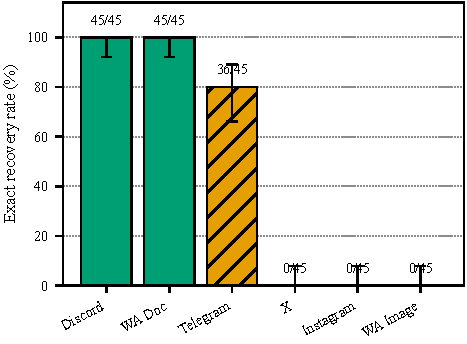
\includegraphics[width=\columnwidth]{paper_figures/fig1_recovery_ci.pdf}
\caption{Exact recovery rate by delivery mode with Wilson 95\% confidence intervals.}
\label{fig:platform}
\end{figure}

Discord and WhatsApp Document achieved 45/45 exact recoveries with zero recorded BER, consistent with byte-preserving file transfer. Telegram recovered 36/45 messages. Its failures are concentrated in cases where platform resizing changes the DCT block registration or where the requested near-capacity payload exceeds the delivered image capacity. Twitter/X, Instagram, and WhatsApp Image recorded 0/45 exact recoveries each and BER 1.0 for every recorded row.

\safeSection{Detailed Channel Analysis}
\safeSubsection{Discord attachment mode}
Discord is the strongest channel in this study. All 45 messages were recovered exactly, including the near-capacity cases. The zero BER result indicates that the attachment path retained the JPEG coefficient stream sufficiently for the native decoder. This does not mean Discord is intrinsically lossless for every client or future policy; it means the tested webhook attachment path did not introduce a transformation that disturbed the selected DCT relationships.

The result is important because the embedding itself is deliberately conservative. ShadowPost does not modify every coefficient, use a perceptual optimization loop, or search for a new synchronization point after delivery. When the original block grid is preserved, the simple relative-order decoder is sufficient. This provides a useful baseline against which all recompressing channels can be compared.

\safeSubsection{WhatsApp document mode}
WhatsApp Document also recovered all 45 messages with zero BER. The document mode is evaluated as file transfer rather than ordinary image presentation: the JPEG remains an attached file instead of being treated as a display image. The outcome supports a practical deployment distinction. A channel may be unsuitable for an image-post workflow while remaining suitable for sending the same JPEG as a file.

The document result should be interpreted together with the image-mode result, not averaged into a generic WhatsApp score. The two modes expose different server behaviors. The document path preserved the encoded structure in all tested rows, while the standard image path failed all fixed-payload trials. For ShadowPost users, selecting the media type is therefore a protocol decision, not a cosmetic choice.

\safeSubsection{Telegram sendPhoto}
Telegram produced the intermediate result, with 36 exact recoveries out of 45 trials. The successful rows show that some returned media remain compatible with the encoder's fixed 8 by 8 block registration. The failed rows show the boundary of that assumption: a transformed derivative can change the number and placement of DCT blocks, so the decoder reads a different coefficient lattice from the one used during embedding.

Telegram failures also illustrate why a single aggregate BER is insufficient. Some failed rows have a measurable BER near one half, consistent with an out-of-registration bit stream; other rows are rejected before transmission because the near-capacity payload is larger than the delivered image can support. These are different engineering failures and should lead to different mitigations.

\begin{figure}[H]
\centering
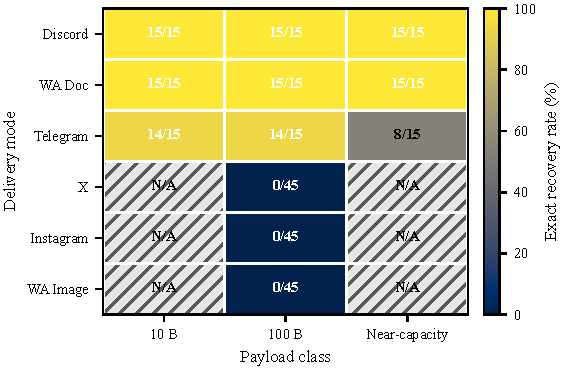
\includegraphics[width=\columnwidth]{paper_figures/fig2_payload_heatmap.pdf}
\caption{Exact recovery by delivery mode and payload class; annotations show recovered trials over total trials, and hatched cells indicate combinations absent from the cohort design.}
\label{fig:payload}
\end{figure}

\safeSubsection{Twitter/X image posts}
The Twitter/X cohort contains 45 fixed 100-byte trials and recovered no messages. Every failed row is recorded with the reproducible fixed-grid extraction failure class. The important observation is that the tested returned media could not be decoded by the current native-grid extractor, even for a short payload.

This result does not establish that every possible X media path is impossible. It establishes that the tested public image-post delivery path is incompatible with the current native-grid decoder. A future design could attempt scale-invariant synchronization, multi-resolution markers, or a spatially re-registered decoder, but those would be new algorithms outside this locked benchmark.

\safeSubsection{Instagram feed posts}
Instagram also recovered 0/45 fixed 100-byte trials. The recorded reasons identify aggressive JPEG transcoding and spatial downsampling. Feed presentation requires the platform to produce display-oriented derivatives, and the derivative is not required to preserve the original JPEG coefficient arrays. As a result, the error-correction layer never receives a stable enough bit stream to operate.

The Instagram outcome is a useful negative control for claims about DCT robustness. DCT-domain embedding is more appropriate than pixel-domain embedding for JPEG workflows, but the transform domain alone does not defeat arbitrary platform resizing. Robustness must be defined relative to a delivery model, and the feed model tested here is substantially more aggressive than a file attachment.

\safeSubsection{WhatsApp standard image mode}
Standard WhatsApp image delivery recovered 0/45 fixed 100-byte trials. The result contrasts sharply with WhatsApp Document and demonstrates that the label ``WhatsApp'' is not a sufficient experimental condition. The media subtype determines whether the system receives an intact JPEG file or a presentation-oriented derivative.

\safeSection{Formal Pipeline and Capacity}
Let $M$ be the plaintext message. ShadowPost first derives a 256-bit key $K$ from a passphrase using scrypt.
\begin{equation}
\text{passphrase}\xrightarrow{\text{scrypt}}K
\end{equation}
AES-GCM then produces ciphertext $C$ and an authentication tag $T$ using a fresh 96-bit nonce $N$.
\begin{equation}
(C,T)=\operatorname{AES\text{-}GCM}_{K}(M,N)
\end{equation}
The framed container is
\begin{equation}
L\,\|\,N\,\|\,C\,\|\,T,
\end{equation}
where $L$ is a two-byte plaintext length field. The framing permits the decoder to distinguish the meaningful message bytes from padding inside the final RS codeword.

The framed byte stream is partitioned into data blocks $D_i$ of 32 bytes.
\begin{equation}
|D_i|=32\ \text{bytes}
\end{equation}
Each $D_i$ is encoded as a 48-byte Reed-Solomon codeword $W_i$.
\begin{equation}
D_i\xrightarrow{\mathrm{RS}(48,32)}W_i,\qquad |W_i|=48\ \text{bytes}
\end{equation}
In the absence of delivery damage, the decoder recovers $W_i$ exactly. With bounded symbol errors, the parity symbols permit correction. When the coefficient grid is displaced, however, the extracted symbols are not local perturbations of $W_i$; they are samples from a different coordinate system, so RS correction may fail or produce an unauthenticated ciphertext.

For an image with $B$ luminance DCT blocks, the two selected pair positions provide four coefficient values per block and two ordering decisions. The raw bit capacity is therefore
\begin{equation}
2B\ \text{bits}
\end{equation}
before framing and code overhead. The available plaintext capacity is smaller because the framed ciphertext, nonce, tag, and RS parity must all fit. For a requested message length $m$, the number of codewords is
\begin{equation}
\left\lceil\frac{2+12+m+16}{32}\right\rceil,
\end{equation}
and the encoded requirement is 48 times that codeword count bytes, or
\begin{equation}
384\left\lceil\frac{2+12+m+16}{32}\right\rceil\ \text{bits}.
\end{equation}

This capacity model explains the near-capacity trials. A payload that fits the original cover may not fit a resized derivative. In such a case, the correct result is a capacity failure, not a BER measurement. The benchmark preserves this distinction by leaving BER empty for trials rejected before delivery.

\safeSection{Error Model and Failure Taxonomy}
The benchmark uses four operational failure classes. A byte-preserving success produces valid extraction, RS decoding, AES-GCM authentication, and exact plaintext equality. A fixed-grid extraction failure means the checked-in native-DCT decoder could not recover a usable stream from the returned media. Reed-Solomon decode and authentication failures are retained as separate classes, while capacity failures identify payloads rejected before a meaningful bit comparison.

A bit error rate is useful only when the decoder can align the received bit positions with the transmitted positions. Under a pure coefficient perturbation model, BER summarizes the damage before RS decoding. Under spatial rescaling, the problem is not merely that individual bits flip; the receiver's index $i$ refers to a different block than the sender's index $i$. This is why several social-feed rows show BER 1.0 and a fixed-grid extraction failure rather than a correctable low BER.

The Telegram rows make this taxonomy concrete. Low or zero BER rows correspond to derivatives that retain a compatible grid. Rows with BER near one half indicate structural desynchronization. Rows with no BER correspond to payloads that exceeded delivered capacity. Treating these categories as one failure class would hide the actual engineering trade-off.

\begin{figure}[H]
\centering
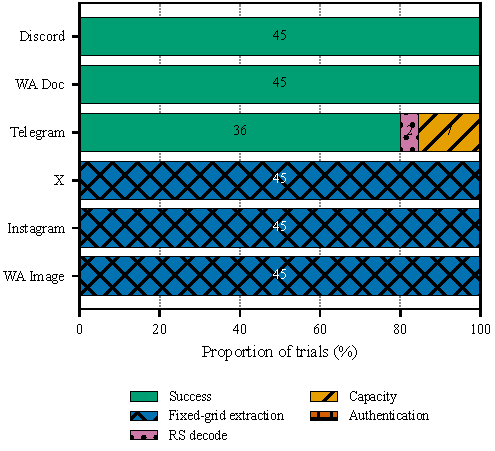
\includegraphics[width=\columnwidth]{paper_figures/fig3_failure_taxonomy.pdf}
\caption{Failure taxonomy by delivery mode, generated from the canonical failure\_reason field. Segment labels show raw trial counts.}
\label{fig:taxonomy}
\end{figure}

Figure~\ref{fig:taxonomy} makes the recorded terminal outcomes explicit. Discord and WhatsApp Document consist entirely of successful trials. Telegram contains 36 successes, seven capacity failures, and two Reed-Solomon decode failures; the canonical CSV contains no Telegram fixed-grid extraction failures. X, Instagram, and WhatsApp Image each contain 45 fixed-grid extraction failures.

\safeSection{Security and Privacy Analysis}
Confidentiality is provided by AES-GCM rather than by the visual concealment layer. An observer who extracts coefficient orderings without the passphrase still obtains ciphertext and cannot recover the authenticated plaintext under the cryptographic assumptions of AES-GCM and scrypt. The nonce is stored with the ciphertext because it is required for decryption but is not secret.

Integrity is equally important. A platform transformation that changes hidden bits should not silently produce a plausible plaintext. GCM authentication rejects modified ciphertext, and the application reports decode failure instead of returning unauthenticated bytes. Reed-Solomon improves availability under bounded corruption but does not replace authentication; corrected data is accepted only after GCM verification.

The system does not claim steganalytic undetectability. Relative coefficient ordering leaves a statistical footprint, and repeated use of the same coefficient positions could be detectable by a sufficiently trained analyst. The contribution evaluated here is delivery survivability under known platform transforms, not resistance to a dedicated detector.

A deployment must also separate passphrases from media distribution. The JPEG can be public while the passphrase remains out of band. Operational security therefore depends on key handling, account security, and the platform's metadata exposure in addition to the DCT payload itself.

\begin{figure*}[!t]
\centering
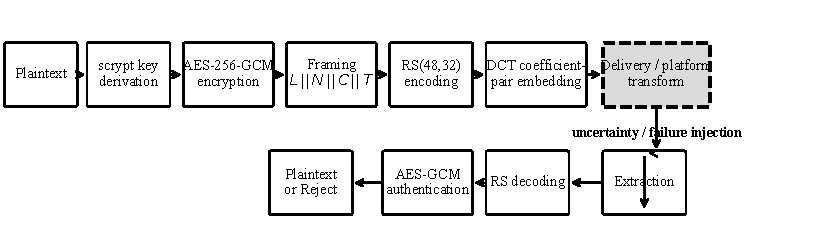
\includegraphics[width=\textwidth]{paper_figures/fig4_system_pipeline.pdf}
\caption{ShadowPost end-to-end system pipeline. The delivery/platform transform is the uncertain stage at which channel-dependent corruption or structural change is introduced.}
\label{fig:pipeline}
\end{figure*}

\safeSection{Reproducibility Procedure}
The repository contains the encoder and decoder, the phase experiments, platform-specific CSVs, the canonical master CSV, charts, and the downloaded Twitter/X and Instagram derivatives. A reproduction should first run the local API round-trip test, then inspect the cover manifest used by the structured cohort. The passphrase and message generator must remain unchanged when comparing results with the stored rows.

For every trial, the reproduction record should include platform mode, trial identifier, source cover or delivered filename, plaintext payload length, success flag, BER when defined, failure reason, and timestamp. These fields make it possible to distinguish a cryptographic failure from a platform transformation and a local preparation error.

The downloaded derivatives should be treated as evidence files, not as new covers. The sender-side stego image and receiver-side delivered image belong to different stages of the experiment. Re-encoding a downloaded derivative before decoding would change the measurement and must be avoided.

The paper generator reads the canonical CSV rather than hard-coding the recovery counts. This keeps the numerical tables coupled to the repository artifact and reduces transcription errors when additional platform trials are added. The generated PDF is therefore a report over a versioned dataset, not an independent hand-edited results sheet.

\safeSection{Comparison with Common Design Alternatives}
Pixel-domain least-significant-bit embedding is simple and can provide useful capacity on an untouched bitmap, but JPEG decoding and recompression operate in a different representation. A platform that decodes and re-encodes the image can erase pixel-level changes even when the visual image appears unchanged. Native-DCT embedding aligns the representation with JPEG compression, which explains the partial Telegram survival and the strong attachment results.

A pure DCT payload without authentication can report a recovered string even when a few bits have changed. ShadowPost instead treats the hidden data as an encrypted authenticated object. This increases overhead, reducing usable capacity, but prevents false-positive recovery and makes the success criterion unambiguous.

A larger error-correcting code could improve recovery under bounded coefficient noise, but it cannot solve arbitrary geometric resampling. Increasing parity would also reduce payload capacity. The current RS(48,32) setting is therefore a controlled baseline, not a claim that the parity rate is globally optimal.

\safeSection{Limitations and Validity Threats}
The benchmark is limited to the accounts, clients, image files, and dates represented by the stored artifacts. Social platforms can change image processing without notice. A later run may produce different dimensions or quantization behavior, so the timestamps and downloaded derivatives are part of the experiment's provenance.

The cohorts are intentionally not collapsed into one perfectly balanced design. The structured cohort tests payload scaling; the feed/media cohort tests a repeated 100-byte message under delivery paths that were already known to produce derivatives. This supports a practical channel comparison but does not support a claim that every platform has been evaluated at every payload size.

The study does not measure peak signal-to-noise ratio, structural similarity, visual quality, computational latency, detector performance, or key-search cost. It also does not evaluate video, animated media, PNG delivery, or alternative client applications. These omissions define the next experimental phase rather than weaknesses that can be hidden by the current success rate.

The Wilson 95\% intervals in Figure~\ref{fig:platform} remain wide with $N=45$ trials per delivery mode. The observed differences are therefore descriptive and suggestive for the tested configurations rather than statistically decisive platform comparisons.

\safeSection{Extended Results Interpretation}
The overall recovery rate of 46.7\% is not a single estimate of algorithm quality. It is the mixture of three channel regimes: two complete-preservation modes, one partially preserving mode, and three zero-recovery feed/image modes. The more useful engineering statement is conditional: when the JPEG structure is preserved, the current pipeline recovered every tested message; when the structure was spatially remapped, it recovered none in the tested rows.

The result also shows why a platform benchmark should report delivery mode explicitly. A product requirement such as ``works on WhatsApp'' is underspecified. The document and image paths have opposite outcomes in this dataset. Similarly, a public feed post is not equivalent to attaching the original JPEG as a file, even if the visual image looks identical to a user.

The main design opportunity is synchronization. A future version could embed a redundant multi-scale marker, infer the delivered block grid from a known cover region, or use a spatial-domain fallback for the scale transform before DCT extraction. Each alternative changes the threat model and must be evaluated separately; none should be silently mixed into the current benchmark.

\safeSection{Discussion}
The results separate two properties that are often conflated: payload robustness and channel preservation. RS parity can correct bounded coefficient errors, but it cannot reconstruct a payload when the receiver loses block-grid alignment or when the platform has replaced the JPEG with a substantially different spatial representation. The 100\% results therefore characterize the tested file-attachment modes, whereas the 0\% feed/image results show that the current native-grid decoder is not invariant to arbitrary rescaling. Telegram occupies an intermediate regime, with some returned media decodable and others failing structurally.

\safeSection{Conclusion}
ShadowPost combines native-JPEG DCT embedding, authenticated encryption, and Reed-Solomon coding in a descriptive delivery-survivability benchmark. Across 270 recorded trials, exact recovery was 46.7\% overall, with complete recovery on the tested Discord attachments and WhatsApp documents, partial recovery on Telegram, and no recovery on the tested X, Instagram, or standard WhatsApp image paths. The central engineering conclusion is direct: error correction helps only while the delivery path preserves enough of the original DCT coordinate system for extraction to remain meaningful.

\appendices
\safeSection{Cover Manifest}
The structured cohort uses the following cover identifiers from the finalized Phase 1 manifest. They span game imagery, vehicles, landscapes, science imagery, particles, and technology scenes, providing variation in texture, edge density, and spatial frequency content.

\begin{table}[H]
\centering
\footnotesize
\begin{tabularx}{\columnwidth}{@{}Y Y@{}}
\toprule
\pathcell{arsenal/preview.jpg} & \pathcell{audiophile/preview.jpg} \\
\pathcell{beach/preview.jpg} & \pathcell{corsair_collection/dotted.fabeb454b273c6d2398a.jpg} \\
\pathcell{deep_space/preview.jpg} & \pathcell{demon_core/preview.jpg} \\
\pathcell{dna_fragment/preview.jpg} & \pathcell{eagleflag/preview.jpg} \\
\pathcell{fantasticcar/preview.jpg} & \pathcell{neon_sunset/preview.jpg} \\
\pathcell{retro/preview.jpg} & \pathcell{ricepod/preview.jpg} \\
\pathcell{sheep/preview.jpg} & \pathcell{shimmering_particles/preview.jpg} \\
\multicolumn{2}{c}{\pathcell{techno/preview.jpg}} \\
\bottomrule
\end{tabularx}
\end{table}

Cover diversity matters because the available DCT coefficients depend on image texture. Smooth areas tend to contain many zero or low-magnitude AC coefficients, while detailed areas distribute energy across more frequencies. A relative-order embedding method may therefore have different visual and robustness behavior on a low-texture sky than on a particle field or a detailed vehicle scene.

The manifest also includes a high-resolution outlier, the Corsair collection image. This cover is useful because it exposes the effect of platform dimension limits. A large original grid offers high sender-side capacity, but a platform may produce a much smaller derivative. The delivered grid, not the source grid, ultimately determines whether extraction can address the encoded bit positions.

The finalized Phase 1 directory is retained as the authoritative embedding manifest. Earlier experimental directories remain historical artifacts and should not be mixed with the final pair-selection results when reproducing the platform benchmark.

\safeSection{Data Dictionary}
The master CSV uses the following fields.
\begin{table}[H]
\centering
\footnotesize
\begin{tabularx}{\columnwidth}{@{}>{\ttfamily\raggedright\arraybackslash\scriptsize}p{0.30\columnwidth}Y@{}}
\toprule
platform & identifies the delivery mode; \\
trial & is the per-mode sequence number; \\
cover\_name & identifies the source or returned media filename; \\
\path{payload_size_bytes} & records the plaintext length requested by the encoder; \\
cover\_width, cover\_height, delivered\_width, and delivered\_height & are dimension fields populated by the automated harness and left empty for historical rows whose manual records did not capture them; \\
success & is true only for exact plaintext recovery; \\
ber & stores the measured bit error rate when alignment and comparison are available; \\
failure\_reason & records a standardized terminal class; \\
timestamp & records the trial event time. \\
\bottomrule
\end{tabularx}
\end{table}

The six platform-specific files are retained beside the canonical master file. A consistency check compares rows grouped by platform and verifies 45 rows per mode. The benchmark is therefore auditable without relying on the generated PDF alone.

A data audit should begin by checking that the master file contains 270 rows and that each platform label occurs exactly 45 times. The sum of true success values must be 126. Discord and WhatsApp Document should each contain 45 successes, Telegram should contain 36, and the remaining three image/feed modes should contain zero. Any mismatch indicates that the paper, chart, or platform-specific files are out of synchronization.

Payload-distribution checks are also required. Discord, Telegram, and WhatsApp Document must each contain fifteen 10-byte rows, fifteen 100-byte rows, and fifteen image-specific near-capacity rows. Twitter/X, Instagram, and WhatsApp Image must each contain forty-five 100-byte rows. This test prevents the fixed-payload feed cohort from being incorrectly described as a three-payload matrix.

BER values require careful handling. An empty BER is not equivalent to zero; it indicates that a meaningful aligned bit comparison was unavailable, commonly because the requested payload could not fit the delivered grid. Aggregate BER should therefore be calculated only over non-empty cells, while the trial still remains a failure in the exact-recovery rate.

Failure reasons are standardized diagnostic labels rather than independent measurements: fixed\_grid\_extraction\_failed, reed\_solomon\_decode\_failed, capacity\_failure, and authentication\_failed. The checked-in scripts assign these classes from decoder outcomes. Reproduction code should preserve the underlying exception or response in its local log where possible, because two rows with the same success flag may require different engineering changes.

The timestamp field provides ordering and provenance but should not be used as a performance measurement. Trial duration was not defined by the stored schema. A future benchmark that evaluates throughput or latency should add explicit start, upload-complete, download-complete, and decode-complete timestamps.

A clean-room reproduction can use the following sequence: verify dependencies; run the local API round trip; load the finalized cover manifest; generate payloads with the locked message function; encode each image once; transmit through the selected mode; retrieve the returned media without additional processing; run extraction and decryption; append one CSV row; and compare the regenerated platform file with the master dataset.

\safeSection{Recommended Future Experiments}
Future work should test the same stego JPEG through multiple clients and image dimensions, record source and delivered dimensions for every row, and separate ordinary recompression from geometric scaling. A second phase should compare fixed-grid extraction with a synchronization-aware decoder. Payload sizes should be normalized across every platform so the effect of capacity can be separated from the effect of delivery transformation.

A stronger evaluation would add visual-quality metrics and a detector study. Embedding strength can be varied while holding the cryptographic and coding layers fixed. The resulting Pareto frontier would show how much imperceptibility is traded for survivability. Repeated measurements over time would also quantify platform drift rather than treating one date as a permanent property of a service.

The first extension should create a balanced cross-platform matrix. Every platform mode should receive the same sender-side stego JPEG for the same cover and payload. This would permit paired comparisons and eliminate ambiguity caused by different delivered filenames or fixed-payload cohorts. The present results remain useful, but a balanced design would support stronger statistical conclusions.

The second extension should isolate transformation type. Controlled tests can independently vary JPEG quality, width, height, chroma subsampling, metadata removal, and cropping. A regression model over these factors could estimate which transform causes the largest loss of synchronization. Live-platform results could then be mapped to the nearest controlled transformation profile.

The third extension should evaluate synchronization-aware extraction. Candidate designs include periodic pilot blocks, repeated sync words at several spatial scales, orientation markers, and a search over plausible delivered dimensions. Each candidate must be compared against the current fixed-grid baseline using identical covers and cryptographic payloads.

The fourth extension should measure detectability. A steganalysis dataset should contain matched cover and stego images generated with several payload rates. Classical rich-model features and modern convolutional detectors can be used to estimate detection accuracy. A survivable system that is trivially detectable would not satisfy the broader covert-communication goal.

The fifth extension should measure perceptual quality with PSNR, SSIM, and a human review protocol. These metrics should be reported before and after platform delivery because a platform can mask sender-side artifacts while simultaneously destroying the payload. Visual similarity alone is therefore not evidence of hidden-message survival.

The sixth extension should evaluate operational reliability. Trials should be repeated across desktop and mobile clients, multiple geographic regions, and several dates. Platform policies change, and a robust engineering conclusion requires confidence intervals over repeated deliveries rather than a single run per prepared image.

Finally, future reports should publish a machine-readable experiment manifest containing software versions, client identifiers, image hashes, source dimensions, delivered dimensions, payload hashes, and decoder version. This would strengthen reproducibility without exposing plaintext secrets or passphrases.

\paperheading{Data Availability and Artifact Map}
The implementation and benchmark artifacts are versioned in the ShadowPost repository. The canonical \texttt{platform\_trials.csv} file is the numerical source for the tables in this paper. Separate CSVs preserve the six delivery-mode subsets. The Phase 1, Phase 2, and Phase 3 directories retain the embedding, error-correction, and encryption experiment outputs used to lock the final pipeline.

The \texttt{downloaded/twitter} and \texttt{downloaded/instagram} directories contain the returned media used by those platform rows. The Phase 7 directory contains generated figures. \texttt{make\_ieee\_paper.py} reads the canonical dataset and produces this PDF, allowing the reported counts to be regenerated from the repository state.

\paperheading{Responsible Use}
Steganography can support legitimate privacy research, watermarking, censorship resistance, and secure metadata-free exchange, but it can also be misused. ShadowPost is presented as a research prototype for measuring image-channel behavior. Deployments should comply with applicable law, institutional policy, and platform terms, and should not be used to conceal harmful activity or bypass authorized monitoring.

\paperheading{Author Contributions and Reproducibility}
The ShadowPost team jointly defined the benchmark objective, selected the delivery modes, and reviewed the interpretation of successful and failed trials. The implementation work covered authenticated payload framing, Reed-Solomon coding, native-JPEG coefficient embedding, extraction, and the platform-trial harness. The evaluation work covered cover-manifest preparation, returned-media collection, CSV validation, chart generation, and manuscript preparation. All authors reviewed the final technical claims and approved the submitted version.

The results are intended to be reproducible from the versioned repository rather than from screenshots or manually transcribed notes. A reproduction should begin with the commit containing the canonical trial CSV, confirm the six platform counts, regenerate the Phase 7 figures, and run the paper generator. The generator reads the master CSV directly, so a changed dataset changes the reported table and aggregate values instead of silently leaving stale numbers in the PDF.

For responsible replication, researchers should preserve the original JPEG bytes, downloaded derivatives, source and delivered dimensions, decoder version, and timestamp for every trial. Platform behavior is operationally variable; repeating the same procedure at a later date or through another client is a new observation, not a correction to the historical result. This distinction keeps the benchmark auditable while avoiding unsupported claims about permanent platform behavior.

\Needspace{20\baselineskip}
\paperheading{Comparative Delivery Summary}
This descriptive table compares the six tested delivery modes under their recorded cohort designs; it is not a universal ranking of the five services.
\begin{table}[H]
\caption{Descriptive comparison of tested delivery modes}
\label{tab:comparison}
\centering
\footnotesize
\begin{tabularx}{\columnwidth}{@{}Y c c Y@{}}
\toprule
Mode & Cohort & Exact & Terminal class \\
\midrule
\ComparisonTableRows
\bottomrule
\end{tabularx}
\end{table}

The media subtype is part of the experimental condition. The tested file-attachment modes completed every trial, Telegram retained most but not all messages, and the three fixed-payload presentation paths produced no exact recoveries. These observations support workflow-specific engineering decisions while leaving other clients, accounts, dates, and upload settings open.

\IEEEtriggeratref{12}
\begin{thebibliography}{14}
\bibitem{b1} W. Bender, D. Gruhl, N. Morimoto, and A. Lu, ``Techniques for data hiding,'' IBM Systems Journal, vol. 35, no. 3-4, pp. 313-336, 1996.
\bibitem{b2} J. Fridrich, Steganography in Digital Media: Principles, Algorithms, and Applications. Cambridge, U.K.: Cambridge University Press, 2009.
\bibitem{b3} National Institute of Standards and Technology, Advanced Encryption Standard (AES), FIPS PUB 197, 2001.
\bibitem{b4} International Telecommunication Union, Information Technology - Digital Compression and Coding of Continuous-Tone Still Images - Requirements and Guidelines, Recommendation T.81, 1992.
\bibitem{b5} I. S. Reed and G. Solomon, ``Polynomial codes over certain finite fields,'' Journal of the Society for Industrial and Applied Mathematics, vol. 8, no. 2, pp. 300-304, 1960.
\bibitem{b6} National Institute of Standards and Technology, Recommendation for Block Cipher Modes of Operation: Galois/Counter Mode (GCM) and GMAC, Special Publication 800-38D, 2007.
\bibitem{b7} C. Cachin, ``An information-theoretic model for steganography,'' in Information Hiding, Lecture Notes in Computer Science, vol. 1525, 1998, pp. 306-318.
\bibitem{b8} N. Provos and P. Honeyman, ``Hide and seek: An introduction to steganography,'' IEEE Security and Privacy, vol. 1, no. 3, pp. 32-44, 2003.
\bibitem{b9} T. Filler, J. Judas, and J. Fridrich, ``Minimizing additive distortion in steganography using syndrome-trellis codes,'' IEEE Transactions on Information Forensics and Security, vol. 6, no. 3, pp. 920-935, 2011.
\bibitem{b10} J. Fridrich and J. Kodovsky, ``Rich models for steganalysis of digital images,'' IEEE Transactions on Information Forensics and Security, vol. 7, no. 3, pp. 868-882, 2012.
\bibitem{b11} C. Percival and S. Josefsson, The scrypt Password-Based Key Derivation Function, IETF RFC 7914, 2016.
\bibitem{b12} ShadowPost Research Team, ``ShadowPost platform trial datasets and implementation,'' project artifact, 2026.
\bibitem{b13} Y. Boroumand, M. Fridrich, and J. Cogranne, ``Deep residual network for steganalysis of digital images,'' IEEE Transactions on Information Forensics and Security, vol. 13, no. 11, pp. 2623-2637, 2018.
\bibitem{b14} V. Holub and J. Fridrich, ``Designing steganographic distortion using directional filters,'' in Proc. IEEE International Workshop on Information Forensics and Security, 2012, pp. 234-239.
\end{thebibliography}
\end{document}
